\chapter{Structure of Software Services} % Main chapter title

\label{Chapter2} % For referencing the chapter elsewhere, use \ref{Chapter1} 

\lhead{Chapter 2. \emph{Structure of Software Services}} % This is for the header on each page - perhaps a shortened title

%----------------------------------------------------------------------------------------

\section{Introduction}

This chapter will present in some detail the structure of the code on each core and how basic services such as inter-core communications, synchronization, task assignments, and fingerprinting are implemented. The data structures for organizing fingerprinting task IDs (FIDs) across the system and how they are communicated to hardware will be shown. The reader is referred back to Figure \ref{f:control_flow} as a reference. Even the simple template code can be difficult to interpret because it is distributed across three cores. Figure \ref{f:control_flow} provides a chronological view of the procedure for dynamic scheduling of a critical task on plain cores by the monitor. The important pieces of code associated with each of these steps will now be discussed.

\begin{figure}
\centering
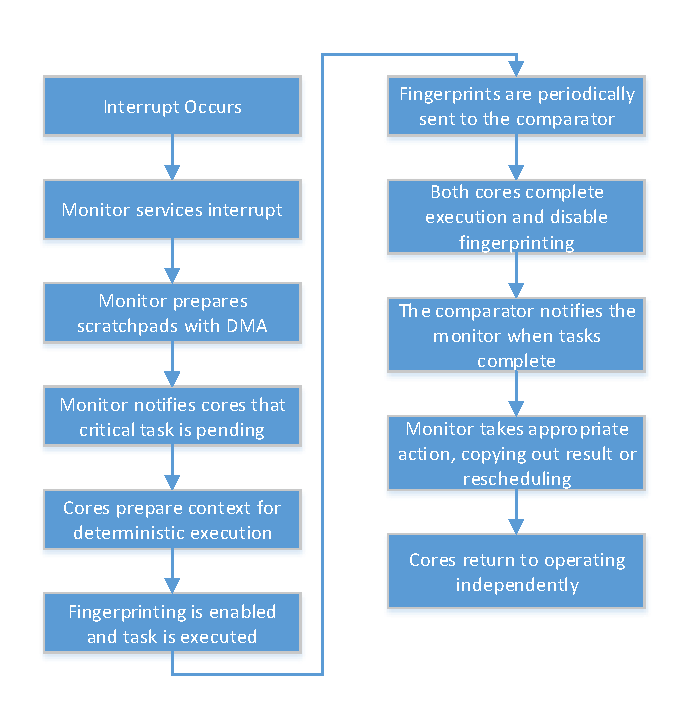
\includegraphics[scale=0.8]{Figures/control_flow}
\caption[Example of directory partitioning]{Example of directory partitioning: Task 0 reserves enough space to maintain a circular queue of size 50. Task 1 reserves a queue of size 25. And Task 2 uses the remainder of available memory.}
\label{f:control_flow}
\end{figure}


\section{Inter-core communication}

As we are dealing with a very simple real-time operating system (RTOS), it is not an easy task to implement a software only solution for message passing between cores. It is not possible to share key data structures such as event-control blocks (ECBs) between cores. An ECB is the basic data structure used by the uC/OS-II RTOS (uCOS from here on) to define mutexes, semaphores, event flags, and queues. Since the RTOS is not built to be able to share ECBs between different instances on different cores it is necessary to develop another solution. Fortunately it is fairly straightforward to create custom memory mappings with soft cores on the FPGA to provide hardware implemented message passing structures.


A 1kB region of memory is reserved for the passing of messages between cores. Furthermore, each core has a register that is addressable by the other cores that triggers an interrupt. The size of the shared memory region can be adjusted if necessary. It is also assumed that each piece of information in the shared memory at any given time is only written by one core. Access to shared memory is controlled with a hardware mutex. Listing \ref{l:mon_init} shows how the monitor core initializes certain system variables and notifies the other cores. The initialization of the plain cores is stalled until the monitor is able to set up certain global variables.

 \begin{lstlisting}[frame=single,language=C,label=l:mon_init,caption={[Monitor passes messages to other cores]The monitor core aquires a hardware mutex and uses shared memory to pass messages to the other cores}] 
 CriticalFunctionPointers* cp = (CriticalFunctionPointers*) SHARED_MEMORY_BASE;
 //Acquire the mutex
altera_avalon_mutex_lock(mutex, 1);
{
	//Set some initial start up values
	cp->critical = critical_task;
	cp->preempt = qsort_test;
	//Notify other cores that initialization is complete
	cp->init_complete = 1;
}//release the mutex
altera_avalon_mutex_unlock(mutex);
 \end{lstlisting}
Meanwhile the plain cores wait for the cp$\rightarrow$ init\_complete variable to change before proceeding with their initialization in Listing \ref{l:core_init}.

\begin{lstlisting}[frame=single,language=C,label=l:core_init,caption={[Plain core startup synchronization]Plain core waits for the initialization by the monitor to finish before updating the variables}] 
//The plain cores wait on the init_complete variable
while(cp->init_complete == 0);
altera_avalon_mutex_lock(mutex, 1);			
{
	//They load the values placed in shared memory by the monitor
	ct = cp->critical;
	pt = cp->preempt;
}
altera_avalon_mutex_unlock(mutex);		
\end{lstlisting}


In this example, the plain cores are at the beginning of their code and are using a spin lock because they all must wait until the monitor has reached a certain point in its startup before they can continue and \emph{no other work} can be done since this is the startup routine. However, \emph{all subsequent} communication between the monitor and the cores will be \emph{interrupt driven}. As previously mentioned, each core is capable of interrupting the execution of the others. Currently, communication is only one way: from the monitor to the plain cores. Listing \ref{l:mon_irq_send} shows the monitor code for causing an interrupt in the other cores and Listing \ref{l:cpu_irq} shows the response from the plain core. This method can be generalized by including a message type header at the beginning of shared memory in order to pass several different types of information. In this example it is assumed that only one type of message passes from monitor to other cores.

\begin{lstlisting}[frame=single,language=C,label=l:mon_irq_send,caption={[Monitor message passing to plain cores]The monitor core puts a message in the shared memory region and then writes to the ISR pointer variables\, triggering interrupts in the other cores.}]
int *isr_0_ptr = (int *) PROCESSOR0_0_CPU_IRQ_0_BASE;
int *isr_1_ptr = (int *) PROCESSOR1_0_CPU_IRQ_0_BASE;	
altera_avalon_mutex_lock(mutex, 1);
{
	cp->task_id0 = (5);
	cp->task_id1 = (5);
	*isr_1_ptr = 1;
	*isr_0_ptr = 1;
}
altera_avalon_mutex_unlock(mutex);
\end{lstlisting}

\begin{lstlisting}[frame=single,language=C,label=l:cpu_irq,caption={[Plain cores retrieve arguments from shared memory]The plain cores handle the interrupt and retrieve the necessary information.}]
static void handle_cpu0_interrupt(void* context) {
	unsigned short task_id;
	altera_avalon_mutex_lock(mutex, 1);
	{
		CriticalFunctionPointers* cp = 
		    (CriticalFunctionPointers*)SHARED_MEMORY_BASE;
		task_id = cp->task_id0;
		*isr_0_ptr = 0;
	}
	altera_avalon_mutex_unlock(mutex);
	if(task_id == CRITICAL_TASK_PRIORITY)
		OSSemPost(mbox);
}
\end{lstlisting}

\section{Initializing and communicating with the Comparator core}

As was already discussed in Chapter \ref{Chapter1}, the monitor core is responsible for organizing the mapping of FIDs to actual critical functions. It is not necessary for this mapping to be static and it is not possible if there are more functions than FIDs. There are two pieces of information required by the comparator in order for it to correctly interpret messages from the fingerprinting units: which core is executing a given FID, and how to partition the local memory space between tasks for the storage of fingerprints.

\subsection{The core assignment table}

The \emph{core assignment table} (CAT) is a mapping of a \emph{physical core ID} (PCID) to a \emph{virtual core ID} (VCID). The PCID is a 4 bit number that is assigned uniquely to each core and fingerprinting unit. The comparator in the current implementation is limited to the comparison of two cores and is not capable of error correction through voting. Furthermore, the FID is a 4 bit number allowing up to 16 concurrent tasks to be fingerprinted. Since each FID can only be executing on two cores at a time, a table keeps track of which two cores are executing each task. An example is shown in Table \ref{t:cat}. Here, the task with FID 0 is defined to execute on cores 0 and 1. The task with FID 1 is defined to execute on cores 1 and 3. The \emph{actual function} associated with each FID can change without changing the CAT. The equivalent code for programming the hardware is shown in Listing \ref{l:cat}.


\begin{table}
\centering
    \begin{tabular}{| l | l | l  |}
    \hline
    Task & PCID 0 & PCID 1\\ \hline
    0 & 0 & 1\\ \hline
    1 & 1 & 3\\ \hline
    2 & 2 & 0\\ \hline
    3 & 2 & 3\\ \hline
    \end{tabular}
    \caption[An example core assignment table.]{An example core assignment table. Each row is associated with a task shown in this picture for demonstration purposes; the real table only has two columns and the task is implicitly defined by the index number. }
    \label{t:cat}
\end{table}


\begin{lstlisting}[frame=single,language=C,label=l:cat,caption=The monitor programs the CAT in the comparator.]
Core_Assignment_Table ca;
//ca.table[VCID][FID] = PCID
ca.table[0][0] = 0;
ca.table[1][0] = 1;
ca.table[0][1] = 1;
ca.table[1][1] = 3;
ca.table[0][2] = 2;
ca.table[1][2] = 0;
ca.table[0][3] = 2;
ca.table[1][3] = 3;
set_core_assignment_table(&ca);
}
\end{lstlisting}

\subsection{Initializing the directory}

The next step for the monitor is to define the partitioning of the comparator's local memory space to store fingerprints. In the current implementation, the comparator has capacity to store 512 fingerprints. The 512 spaces can be divided amongst the 16 FIDs in arbitrarily sized circular queues. For instance, suppose FID 1 is associated with a function known to produce a single fingerprint. It is possible to reserve a single memory location for this task. Suppose FID 1 is known to produce over a thousand fingerprints. It may be prudent to subdivide this task into several fingerprinting intervals. However it is also possible to reserve a queue of size 50 for this task if it can be shown that the fingerprint buffer will not overflow (due to one core executing significantly faster than the other). Development of a feedback mechanism to slow down a core that is pulling too far ahead of its partner core without explicit software barriers is under way. One method of setting the directory according to this example is shown in Listing \ref{l:dir_init}. It is crucial to \emph{never} make changes to the directory structure while any tasks are being fingerprinted. For now it is the case that both virtual cores require the same directory layout, however it is still necessary to set the directory for each core individually. An example of directory partitioning is shown in Figure \ref{f:directory}

\begin{lstlisting}[frame=single,language=C,label=l:dir_init,caption=Initializing the Comparator directory.]
Directory_Init_Struct d;
//Set the directory for each virtual core
for(i = 0; i < 2; i++){
	d.core_id = i;
	//Task 0 requires a single slot
	d.key = 0;
	d.start_ptr = 0;
	d.end_ptr = 0;
	set_task_directory(&d);
	//task 1 requires several slots
	d.start_ptr = 1;
	d.end_ptr = 51;
	set_task_directory(&d);
}
\end{lstlisting}


\begin{figure}[ht]
\centering
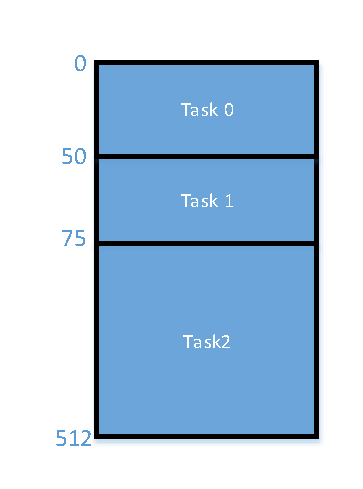
\includegraphics[scale=0.8]{Figures/directory}
\caption[Example of directory partitioning]{Example of directory partitioning: Task 0 reserves enough space to maintain a circular queue of size 50. Task 1 reserves a queue of size 25. And Task 2 uses the remainder of available memory.}
\label{f:directory}
\end{figure}

\section{Initiating a critical task with the Monitor}
Once the comparator has been properly initialized, the Monitor can begin to request the execution of critical tasks from the plain cores. Presumably the request from the monitor would itself be triggered by some interrupt. The monitor will then acquire the hardware mutex, transfer any necessary information into the scratchpads of the cores using DMA, place a pointer to the function, the FID, and any other arguments that can be user defined in shared memory, and interrupt the cores. Listing \ref{l:mon_task} shows how the monitor might initiate a critical task.
\begin{lstlisting}[frame=single,language=C,label=l:mon_task,caption={[Mointor initiates a critical task on plain cores]The monitor requests cores 0 and 1 to begin executing a function called critical\_task with FID 0.}]
altera_avalon_mutex_lock(mutex, 1);
{
	cp->function[0] = critical_task;
	cp->function[1] = critical_task;	
	cp->fid[0] = (0);
	cp->fid[1] = (0);	
	cp->blocksize[0] = 0x5ff;
	cp->blocksize[1] = 0x5ff;
	cp->args[0] = (void*)function_args;
	cp->args[1] = (void*)function_args;
	*irq_1_ptr = 1;
	*irq_0_ptr = 1;
}
altera_avalon_mutex_unlock(mutex);
\end{lstlisting}
\section{Executing a critical task with fingerprinting}
uCOS has a capacity for 256 tasks with priorities 0-255. It is not possible for two tasks to have the same priority. The simplest thing to do is to reserve tasks 0-15 for fingerprinting. Each OS task (OST) is assigned a generic wrapper that will execute an arbitrary function associated with the given FID. The identities of the function and FID are passed by the comparator as shown in Listing \ref{l:mon_task}. More flexible and powerful message passing schemes can be implemented. The method of responding to a request from the monitor is shown in listing \ref{l:cpu_response}. Some parts of the code not essential to the current discussion have been omitted.
\begin{lstlisting}[frame=single,language=C,label=l:cpu_response,caption=Plain core 0 responds to the request from the monitor.]
void (*critical_task)(void*);
int blocksize;
//Interrupt handler
static void handle_cpu0_interrupt(void* context) {
	unsigned short task_id;
	altera_avalon_mutex_lock(mutex, 1);
	{
        CriticalFunctionPointers* cp = 
            (CriticalFunctionPointers*)SHARED_MEMORY_BASE;
        //retrieve the FID of the task
		task_id = cp->fid[0];
		//retrieve the address of the function
		critical_task = cp->function[0]
		//retrieve the fingerprinting block size
		blocksize = cp->blocksize[0];
		//reset the IRQ
		*irq_0_ptr = 0;
	}
	altera_avalon_mutex_unlock(mutex);
	//Activate the appropriate OS task
	if(task_id == PRIORITY_0)
		OSSemPost(sem_0);
	else if(task_id == PRIORITY_1)
		OSSemPost(sem_1);
}

//The tlb must be used for global variable references
void init_tlb(){
	set_cputable_entry(1, GLOBAL_VARIABLE_SECTION);
	set_spmtable_entry(1, TLB_BASE);

	//Enable the translations
	set_enable(0x2);

}

//The critical task wrapper:
INT8U err;
void critical_task_wrapper(void* pdata){
	int* p = pdata;
    //The priority is assigned to the task when created by the OS
	int priority = *p;
	while(1){
		//A single task wrapper can be written for all priorities using
		//conditional waiting
		if(priority == PRIORITY_0)
			OSSemPend(sem_0, 0, &err);
		else if(priority == PRIORITY_1)
			OSSemPend(sem_1, 0, &err);
	    
	    //the critical task address is loaded onto the stack
	    void (*pt)(int) = critical_task;
		//the block size is forwarded to the fingerprint unit	    
	    fprint_set_block_size(blocksize);
	    //The TLB is initialized with the proper translation table
		init_tlb();
		//The TLB is enabled
	    enable_tlb();
		long registers[8];
		//The callee saved registers must be pushed to the stack
		// and set to 0
		context_switch(registers);
		//The global pointer is set to match the monitor core
		set_gp();
		//The critical task is executed
		critical_task(&args);
		//Restore the local global pointer register
		restore_gp();
		//Restore the callee saved registers
		context_restore(registers);
		//Turn off translation
		disable_tlb();
	}
}
\end{lstlisting}

There are several important things that happen in this code. First is the interrupt handler. This retrieves the FID and the function pointer from the shared memory region. It also retrieves the blocksize that sets the number of stores used by the fingerprint unit to calculate each fingerprint (where the size of the block affects the hamming distance and guaranteed error coverage provided by the CRC algorithm). It then signals the appropriate task wrapper based on the value of the FID. The task wrapper is the same generic wrapper for all critical tasks. Each wrapper is statically assigned a priority by the OS during startup. Each wrapper waits on its own signal. When the signal arrives from the interrupt handler, the wrapper then does several things before calling the task: it turns on the TLB, it saves and resets the context, it changes the global pointer, and then it finally calls the critical task. Recall that memory translation, GP substitution, and the setting of callee saved registers to zero prior to initiating fingerprinting are required to ensure \emph{deterministic execution}. Also note that changes are made to the initial interrupt context save routine in order to restore the GP for interrupt handlers so that these will not be broken if interrupts are not disabled during the critical task.

There is one more layer to get to the proper critical function. The issue is that fingerprinting must be enabled and disabled without storing the return address of the local wrapper function. This return address would not match on the different cores. Therefore a \emph{wrapper within the wrapper} is required. The code that enables and disables fingerprinting must be part of the shared code. Suppose that the critical task in question was an FSM control for the shift logic in a car. When the critical task is called from the wrapper in Listing \ref{l:cpu_response}, it takes the form of Listing \ref{l:critical_task}. This code, including the FSM function, are compiled for the Monitor to ensure the location of global variables are in the section of memory being translated by the TLB.

\begin{lstlisting}[frame=single,language=C,label=l:critical_task,caption=The inner layer wrapper.]
void critical_task(void* args){
	int priority = *(int *)args;
	enable_fprint_task(priority);
	    ShiftLogic_step();
	disable_fprint_task(priority);
}
\end{lstlisting}

All other activity between the fingerprinting units themselves and the comparator are invisible to the software. When the result of a comparison is ready, the Monitor is notified via interrupt. As shown in Listing \ref{l:mon_comp_int}, the Monitor uses simple functions to retrieve a status update from the Comparator. Depending on the program, further actions can be taken. It remains to be done to develop a generalized framework across the system for killing and restarting failed tasks.

\begin{lstlisting}[frame=single,language=C,label=l:mon_comp_int,caption=The monitor interrupt handler for the comparator]
static void handle_comp_interrupt(void* context) {
	int endstate[10];
	Fprint_Status status;
	fprint_status(&status);
	...
}
\end{lstlisting}